\documentclass[11pt, a4paper]{report}

\usepackage[french]{babel}
\usepackage{float}
\usepackage{stackengine}
\usepackage{minted}
\usepackage{wrapfig}

\title{Projet ORA}
\team{Crab Wave}
\author{leo.benito  •  raffael.moraisin  •  adam.thibert  •  pierre-corentin.auger}
\university{EPITA}
\date{6 mars 2020}
\email{contact@crabwave.com}
\homepage{https://ora.crabwave.com}
\github{https://github.com/Crab-Wave}

\logo{assets/logo.png}
\firstpage{assets/firstpage.png}
\background{assets/background.png}

\lheader{Rapport de soutenance}
\rheader{Projet ORA}

\restylefloat{table}

\urlstyle{same}
\newcommand*{\surl}[1]{{\bodyfont\color{clearocean}\selectfont\url{#1}}}

\renewcommand\cftsecfont{\Large\color{orangecrab}\bfseries}
\renewcommand\cftsubsecfont{\large\color{bluewave}\bfseries}
\renewcommand\cftsubsubsecfont{\normalsize\color{darkora}\bfseries}

\begin{document}
  \maketitle
  \thispagestyle{empty}   %% Remove page number
  \clearpage
 
  \tableofcontents
  \thispagestyle{empty}
  \clearpage

  \section{Introduction}
    \subsection{Présentation de ORA}
    ORA est une application de stockage de fichiers en \textit{Peer-to-Peer}, centrée autour de la notion de partage de fichiers au sein d'un même groupe. Le \textit{Peer-to-Peer} est un modèle de réseau informatique où, contrairement au modèle client-serveur où il y a un seul serveur, chaque client est aussi un serveur. Cette technologie va donc nous permettre de partager nos fichiers sans passer par un tiers.\newline

    Nous avons défini un vocabulaire spécifique à notre application. Afin de bien comprendre la suite ce document, voici la définition des principales notions:
    \begin{itemize}
        \item les utilisateurs seront appelés des \textbf{Identities}
        \item les machines utilisées par ces derniers seront appelées des \textbf{Nodes}
        \item les groupes de Nodes partageant des fichiers seront appelés des \textbf{Clusters}
    \end{itemize}
    \bigbreak
    
    Cette application a pour but de fonctionner sous Windows comme spécifié dans le dossier distribué mais aussi compatible avec Linux car ce système d'exploitation nous tient particulièrement à coeur.
    Aussi la thématique de la sécurité est importante pour nous, l'application utilise le chiffrement RSA afin de sécuriser les données car des fichiers personnels peuvent être partagés. De plus, si vous n'avez tout de même pas confiance en le Tracker hébergé par notre équipe, vous pouvez tout à fait héberger votre propre instance d'un Tracker ORA et même en modifier le code !
    En effet, ORA vise à être totalement open-source à terme, ce qui permet à n'importe qui d'en créer une version modifiée et de la redistribuer. Notre projet contient deux implémentations différentes de l'API qui auraient pu être créées par des développeurs utilisant celle de ORA. La première implémentation est le CLI, l'application en lignes de commandes dont le développement a débuté afin de fournir un aperçu de l'interaction avec le Tracker. La deuxième est le GUI, l'application graphique qui est plus \textit{end-user friendly} dont le développement commencera après la première soutenance. Ces deux implémentations nous permettent de montrer que grâce à l'API ont peux gérer les fichiers, Clusters et Nodes de manière totalement différente.

    \clearpage
    \subsection{Division du projet}
Comme mentionné dans le cahier des charges nous avons divisé le projet en plusieurs sous-projets. Cette division permet notamment une séparation entre le Core et les applications CLI et GUI. Cette séparation permet notamment à d'autres développeurs de créer leurs propres applications basées sur l'API de ORA. Étant nous même développeurs, la possibilité de construire notre propre application sur une API de cette manière nous tient particulièrement à coeur.\newline

    Le découpage du projet est donc le suivant:
    \begin{itemize}
      \item \textbf{Tracker} le programme permettant de connecter les différents pairs.
      \item \textbf{API} (\textit{Application Programming Interface}) contenant un ensemble normalisé de classes, de méthodes, de fonctions et de constantes servant de façade aux applications voulant utiliser ORA (CLI, GUI, etc \ldots).
      \item \textbf{Core} contenant toutes les implémentations des classes, méthodes et fonctions définies dans l'\textbf{API}.
      \item \textbf{Daemon} contenant l'application principale s'exécutant en arrière-plan, se basant sur les fonctionnalités du \textbf{Core} .
      \item \textbf{Application CLI} contenant l'outil en lignes de commandes servant à interagir avec les fonctionnalités du programme.
      \item \textbf{Application GUI} contenant l'outil en interface graphique servant à interagir avec les fonctionnalités du programme.
      \item \textbf{Site Web} nécessaire pour la communication avec les utilisateurs (téléchargement du programme, présentation du projet, etc \ldots).
    \end{itemize}
    \bigbreak

    \subsection{Planning de réalisation}
Voici le planning de réalisation qui a été présenté dans le cahier des charges:

\begin{table}[H]
\centering
\scalebox{1.5}{\begin{tabular}{llll} \hline
\multicolumn{1}{|l|}{Tâches}   & \multicolumn{1}{l|}{1}    & \multicolumn{1}{l|}{2}    & \multicolumn{1}{l|}{3}    \\ \hline
\multicolumn{1}{|l|}{Tracker}  & \multicolumn{1}{l|}{70\%} & \multicolumn{1}{l|}{90\%} & \multicolumn{1}{l|}{100\%} \\ \hline
\multicolumn{1}{|l|}{API}      & \multicolumn{1}{l|}{50\%} & \multicolumn{1}{l|}{80\%} & \multicolumn{1}{l|}{100\%} \\ \hline
\multicolumn{1}{|l|}{Core}     & \multicolumn{1}{l|}{40\%} & \multicolumn{1}{l|}{70\%} & \multicolumn{1}{l|}{100\%} \\ \hline
\multicolumn{1}{|l|}{Daemon}   & \multicolumn{1}{l|}{10\%} & \multicolumn{1}{l|}{50\%} & \multicolumn{1}{l|}{100\%} \\ \hline
\multicolumn{1}{|l|}{CLI}      & \multicolumn{1}{l|}{20\%} & \multicolumn{1}{l|}{80\%} & \multicolumn{1}{l|}{100\%} \\ \hline
\multicolumn{1}{|l|}{GUI}      & \multicolumn{1}{l|}{0\%}  & \multicolumn{1}{l|}{30\%} & \multicolumn{1}{l|}{100\%} \\ \hline
\multicolumn{1}{|l|}{Site Web} & \multicolumn{1}{l|}{40\%} & \multicolumn{1}{l|}{70\%} & \multicolumn{1}{l|}{100\%} \\ \hline
\multicolumn{1}{|l|}{\LaTeX}   & \multicolumn{1}{l|}{40\%} & \multicolumn{1}{l|}{70\%} & \multicolumn{1}{l|}{100\%} \\ \hline
\end{tabular}}
\end{table}

Nous expliquerons dans la partie \textbf{Avancement} ce qui a été fait depuis le début du projet, et dans la partie \textbf{Prochaine Soutenance} ce qui sera à faire d'ici la semaine du 20 avril.

    \subsection{Répartition des tâches}
Voici le tableau de la répartition des tâches qui a été présenté dans le cahier des charges:

\begin{table}[H]
\centering
\scalebox{1.5}{\begin{tabular}{|l|l|l|}
\hline
\textbf{Tâche}         & \textbf{Responsable} & \textbf{Suppléant} \\ \hline
Tracker                & Léo                  & Raffaël            \\ \hline
API                    & Léo                  & Adam               \\ \hline
Core - Networking      & Adam                 & Léo                \\ \hline
Core - Chiffrement     & Pierre-Corentin      & Raffaël            \\ \hline
Core - Compression     & Pierre-Corentin      & Adam               \\ \hline
Core - File Management & Raffaël              & Léo                \\ \hline
Daemon                 & Adam                 & Raffaël            \\ \hline
Application - CLI      & Raffaël              & Pierre-Corentin    \\ \hline
Application - GUI      & Raffaël              & Léo                \\ \hline
Site Web               & Léo                  & Pierre-Corentin    \\ \hline
\LaTeX                 & Adam                 & Pierre-Corentin    \\ \hline
\end{tabular}}
\end{table}

\clearpage

  \section{Avancement}
Dans cette partie, nous détaillerons ce qui a été réalisé depuis la validation du cahier des charges.

    \subsection{Tracker}
      Le Tracker étant le programme qui permet de mettre en connexion les différents Nodes, il nous fallait un serveur utilisant un protocole garantissant la réception des paquets. Ainsi, nous avons choisi de partir sur un protocole basé sur \textit{TCP}. Les requêtes au Tracker étant légères et afin de garder une simplicité d'utilisation (pour les développeurs souhaitant créer une application basée sur le Tracker de ORA) nous avons choisi que le Tracker serait un serveur \textit{HTTP} fonctionnant sous forme d'\textit{API RESTful}. Le serveur est non bloquant c'est-à-dire qu'il peut traiter plusieurs requêtes en même temps sans avoir à attendre la fin du traitement de la requête précédente. En effet, le Tracker aurait été inutilisable si on devait attendre que le traitement de la requête du client précédent soit fini avant de pouvoir espérer recevoir une réponse à sa requête. Pour pouvoir renvoyer des informations sur les Clusters par exemple, il est nécessaire de stocker ces informations. Afin de les stocker, nous avons utilisé la base de donnée \textit{LevelDB} développée par Google, qui est réputée pour sa vitesse et sa faible taille sur le disque. Aussi, l'architecture modulaire que nous avons choisi pour le Tracker nous permet de rajouter des routes et des modèles de données simplement tout en conservant un serveur performant.
      \bigskip
      Les \textit{endpoints} (point d'accès) actuellement implémentés sont:
      \begin{itemize}
          \item \verb|GET /| --- renvoie un message de bienvenue.
          \item \verb|GET /clusters/unIdentifiant| --- renvoie les informations associées aux Cluster ayant pour identifiant \verb|unIdentifiant|.
          \item \verb|POST /clusters?name=unNom| --- crée un Cluster dont le nom est \verb|unNom| et renvoi son identifiant.
          \item \verb|DELETE /clusters/unIdentifiant| --- supprime le Cluster associé à l'identifiant \verb|unIdentifiant|.
      \end{itemize}
      \bigskip

      Sachant que toute requête à un \textit{endpoint} non spécifié ici renverra une réponse dont le code HTTP sera 4XX.
      Cependant il y a un problème auquel nous n'avions pas pensé lors de la rédaction du cahier des charges: il faut authentifier les routes du Tracker. En effet, nous ne voulons pas que n'importe qui puisse supprimer n'importe quel Cluster. Nous souhaitons que seul le propriétaire du Cluster puisse effectuer cette action. Il faut donc authentifier le Node qui fait la requête au Tracker afin de déterminer si c'est bel et bien le propriétaire.\newline

      Enfin, le Tracker est actuellement disponible à l'adresse suivante: \surl{https://tracker.ora.crabwave.com}.

      \begin{figure}[H]
        \centering
        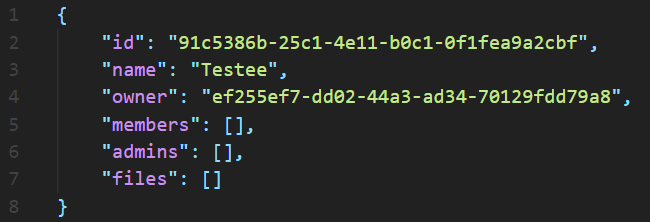
\includegraphics[width=15cm]{assets/presentation1/tracker_request.png}
        \caption{Exemple de réponse du Tracker à une requête GET /clusters/id}
      \end{figure}
    
    \subsection{Daemon}
      Le projet du Daemon à été créé et certaines librairies nécessaires à son fonctionnement ont été importées mais aucun code réel n'a été produit. Le programme n'est donc pour l'instant pas du tout fonctionnel bien que des recherches aient été effectuées.

    \subsection{API (\textit{Application Programming Interface})}
      \begin{wrapfigure}{o}{0cm}
        \centering
        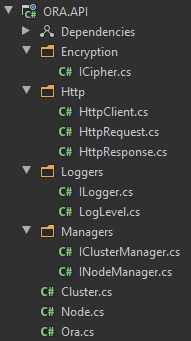
\includegraphics[height=9cm]{assets/presentation1/api.png}
        \caption{Architecture du projet \textit{API}}
      \end{wrapfigure}
      De manière à correctement structurer le projet, nous avons décidé de couper celui-ci en 2 parties distinctes, l'API qui définit l'architecture globale du projet, les méthodes ainsi que les structures qu'elles utilisent (comme les Cluster, les Nodes, etc\ldots), et le Core qui implémente ces méthodes et structures de données. De plus, l'API étant totalement indépendante d'une quelconque implémentation, cela permet à n'importe qui de venir étendre les fonctionnalités d'ORA en implémentant les fonctionnalités voulues mais aussi à n'importe quel développeur de ne pas se soucier du support de différentes plateformes et de se focaliser uniquement sur l'utilisation de cette interface.\newline
      Nous avons donc créer plusieurs structures à ce jour:
      \begin{itemize}
          \item \textit{ICipher}, représentant un objet de chiffrement;
          \item \textit{ILogger}, permettant de gérer les traces générées par ORA (que ce soit pour du debuggage ou bien des erreurs);
          \item \textit{HttpClient}, représentant un client HTTP basique capable de faire des requêtes GET/POST/DELETE/PUT;
          \item \textit{IClusterManager}, permettant de gérer la création/suppression de Clusters;
          \item \textit{INodeManager}, permettant de gérer la création/suppression de Nodes;
          \item \textit{Les autres structures sont présentes car nécessaire à celles définies plus haut}.
      \end{itemize}

    \subsection{Core}
    
      \subsubsection{Client HTTP}
        Afin de communiquer avec le Tracker, nous avons eu besoin d'un client HTTP fonctionnel implémentant la classe disponible dans l'API. Nous en avons donc implémenté un grâce à la librairie Unirest qui permet de créer des requêtes HTTP assez simplement en quelques lignes seulement.
        
\clearpage

      \subsubsection{Chiffrement}
      Afin de garantir la sécurité des échanges entre utilisateurs, nous avons créé une classe permettant de chiffrer des données en utilisant l'algorithme \textit{RSA}.\newline
      .NET ayant déjà un espace de nom permettant de chiffrer des données, nommé
      \textit{System.Security.Cryptography}, nous nous en sommes servis. Nous avons utilisé la classe \textit{RSACryptoServiceProvider} de cet espace de nom. La classe crée permet à l'utilisateur de choisir la taille de sa clé et comporte 2 méthodes :
      \begin{itemize}
          \item \textit{Encrypt}, qui chiffre les données;
          \item \textit{Decrypt}, qui déchiffre les données.
      \end{itemize}
      \bigbreak
    
      Nous avions dans un premier temps considéré l'utilisation de la classe \textit{CspParameters} afin de stocker les clés dans un conteneur, mais cela aurait rendu l'application incompatible avec Linux.

    \begin{figure}[H]
        \centering
        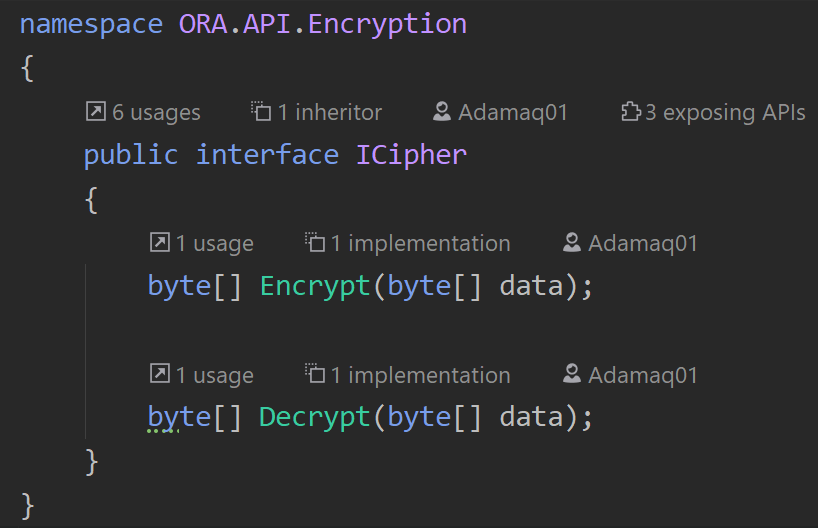
\includegraphics[width=15cm]{assets/presentation1/cipher_interface.png}
        \caption{Interface du \textit{Chiffrement}}
    \end{figure}
        
    \clearpage

      \subsubsection{Data Management}
        Pour pouvoir introduire la notion de \textit{Data Management}, nous avons tout d'abord dû implémenter des Clusters pour réaliser celui-ci.\newline
        Ces derniers sont des groupes dans lesquels des identités (utilisateurs) possédant plusieurs \textit{Nodes} (machines) pourront échanger leurs fichiers ou leurs dossiers entre eux grâce à la technologie \textit{Peer-to-Peer}.\newline
        
        Ainsi nous avons codé trois méthodes sur une interface afin de manipuler ces Clusters :
        \begin{itemize}
              \item \textit{CreateCluster} qui permet d'en ajouter un;
              \item \textit{GetCluster} qui permet d'en avoir un déjà existant;
              \item \textit{DeleteCluster} qui permet d'en supprimer un si cela est possible.
          \end{itemize}

          \begin{figure}[H]
            \centering
            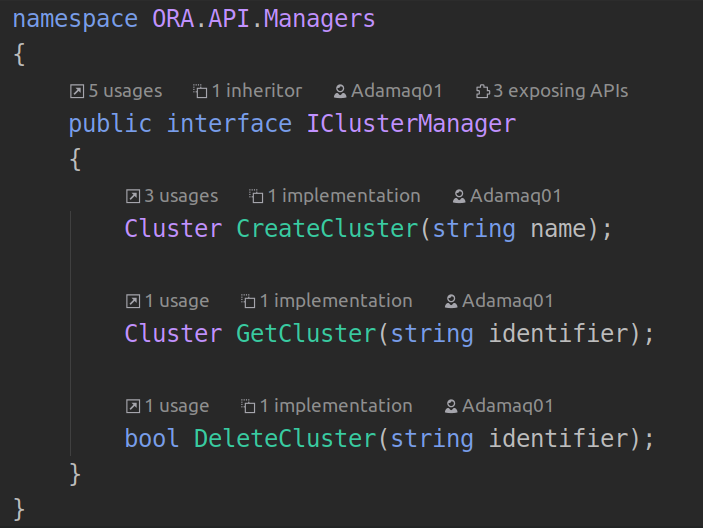
\includegraphics[width=15cm]{assets/presentation1/cluster_interface.png}
            \caption{Interface du Cluster Management}
          \end{figure}
          
    \clearpage
          
    \subsection{Site Web}
      Aujourd'hui un site web est un élément indispensable à tout projet afin de le promouvoir ou de le présenter d'une manière claire et précise. Cependant, notre site web contiendra aussi la documentation de l'API et du Tracker afin d'aider les développeurs à réaliser leurs applications basées sur ORA.\newline

      Afin de réaliser le frontend de ce site nous avons utilisé la bibliothèque React.js pour créer un site web dynamique en Javascript, ainsi que la bibliothèque Sass qui permet, entre autres, d'écrire des feuilles de style de manière plus simple et élégante. Nous n'avons pas développé de backend pour ce site étant donné que nous n'en voyons pas l'utilité. Pour l'hébergement du site web, nous avons utilisé now.sh de ZEIT à la place de Netlify (mentionné dans le cahier des charges) qui est totalement gratuit et qui permet à chaque membre du groupe d'avoir des accès d'administration sur le site. Nous avons aussi acheté le nom de domaine \surl{crabwave.com}. Ainsi, le site web est disponible à l'adresse suivante: \surl{https://ora.crabwave.com}.\newline

      Le site web de ORA est découpé en deux grosses parties:
      \begin{itemize}
        \item La page principale, qui contient la présentation du projet, la liste des membres du groupe ainsi que les liens de téléchargement du projet;
        \item La page de documentation, contenant les présentations de l'API et du Tracker, qui va aider les développeurs à créer leurs propres applications basées sur ORA.
      \end{itemize}
      \bigbreak
    
      \begin{figure}[H]
        \centering
        
\includegraphics[width=17cm]{assets/presentation1/website_screenshots/home.png}
        \caption{Accueil de la page principale}
      \end{figure}
      \begin{figure}[H]
        \centering
        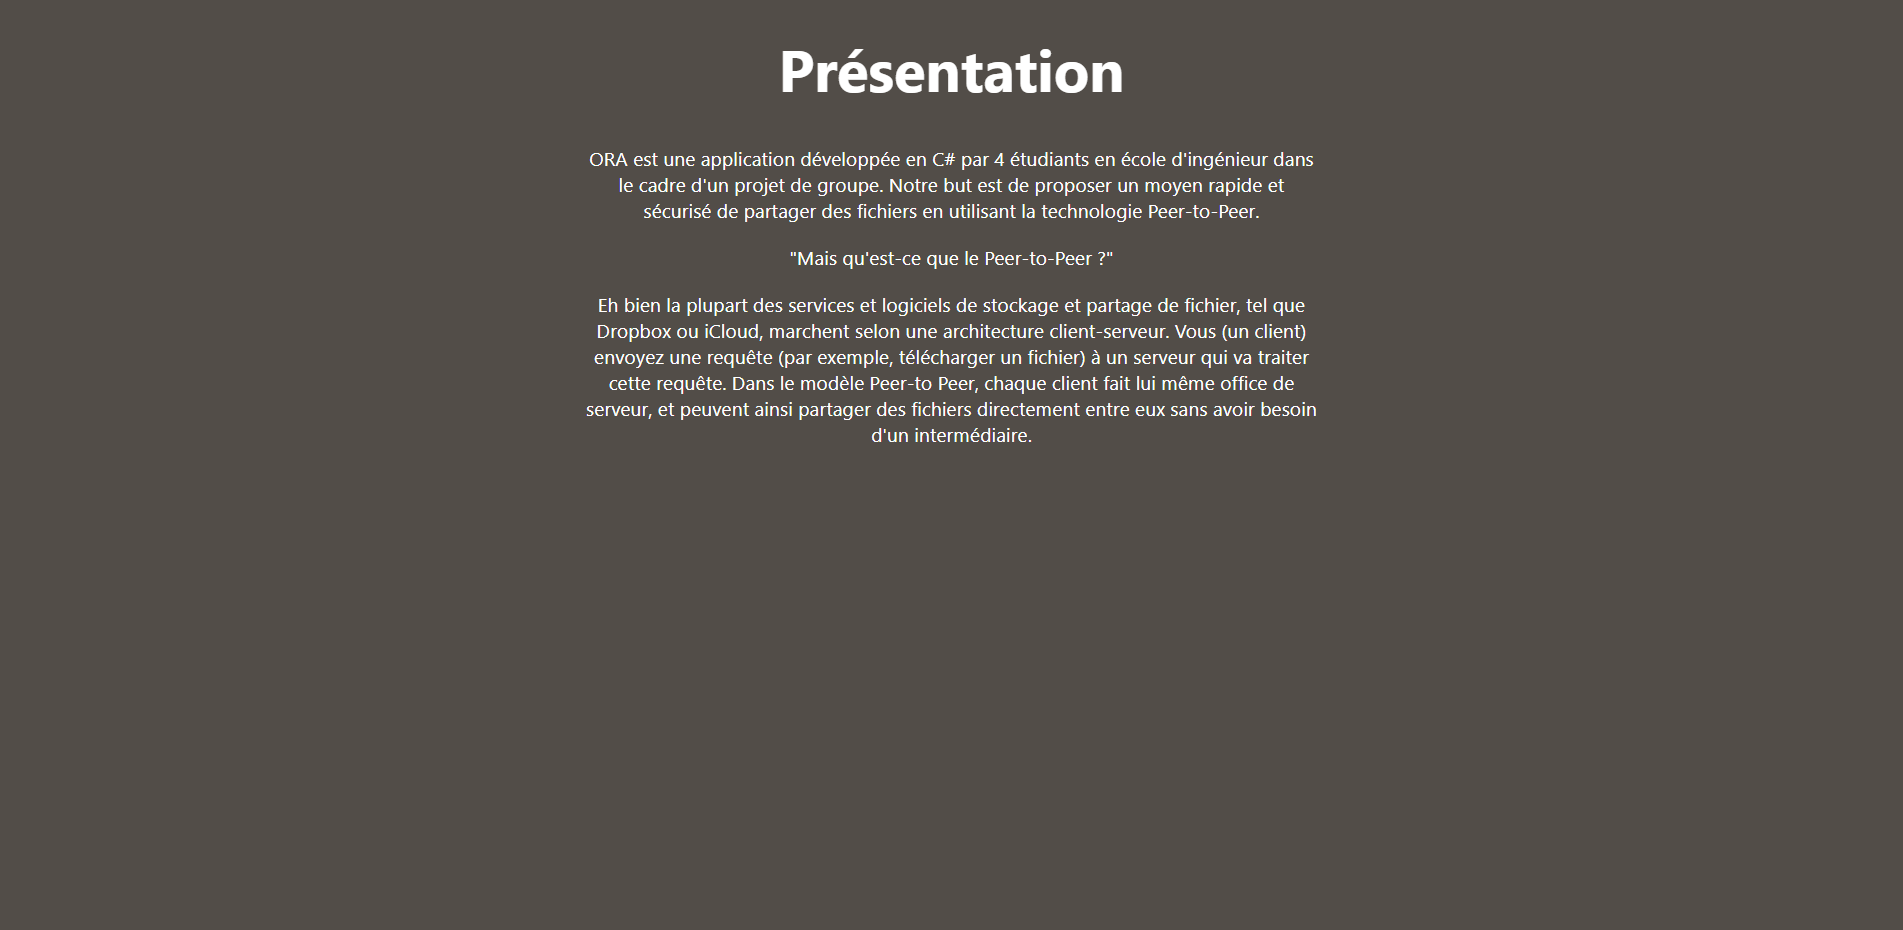
\includegraphics[width=17cm]{assets/presentation1/website_screenshots/presentation.png}
        \caption{Présentation du projet}
      \end{figure}
      \begin{figure}[H]
        \centering
        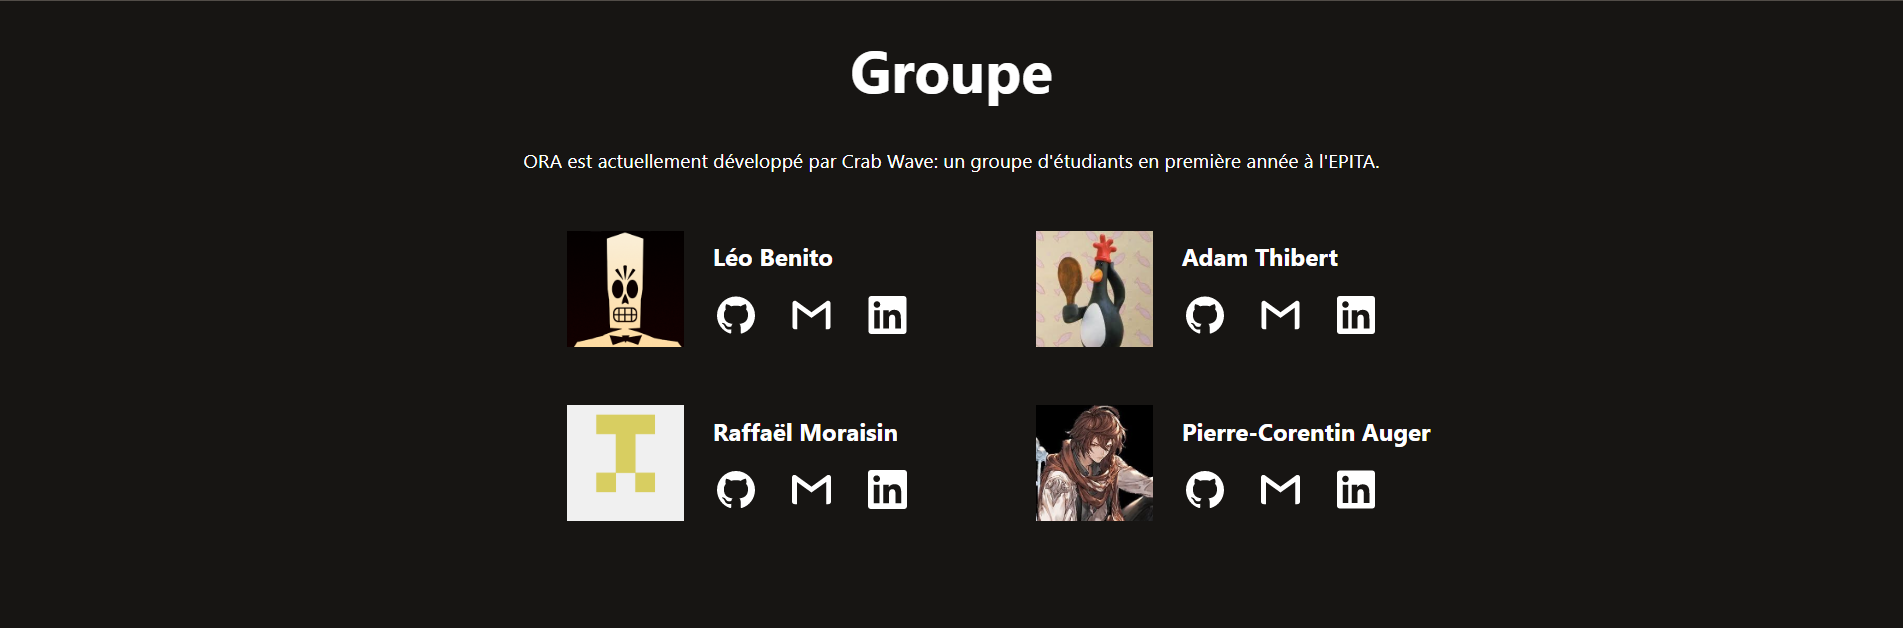
\includegraphics[width=17cm]{assets/presentation1/website_screenshots/group.png}
        \caption{Présentation des membres du groupe}
      \end{figure}
      \begin{figure}[H]
        \centering
        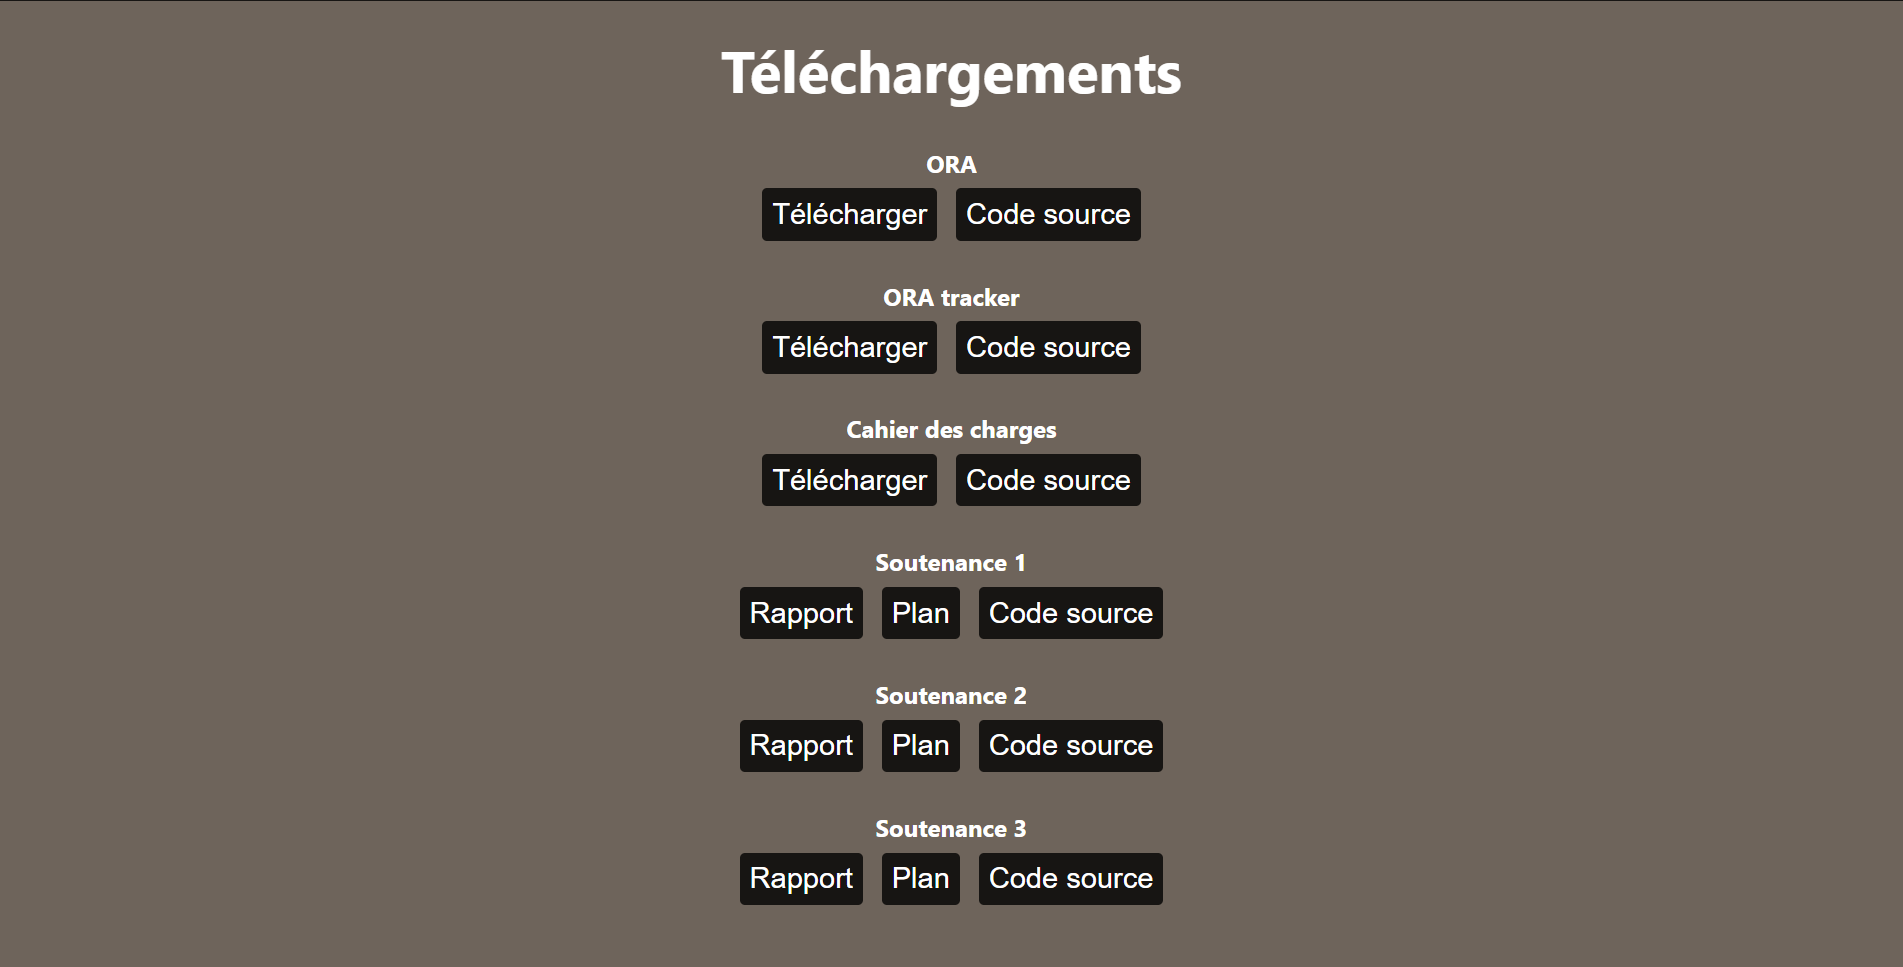
\includegraphics[width=17cm]{assets/presentation1/website_screenshots/downloads.png}
        \caption{Lien de téléchargement des fichiers du projet}
      \end{figure}
      \begin{figure}[H]
        \centering
        
\includegraphics[width=17cm]{assets/presentation1/website_screenshots/contact.png}
        \caption{Moyens de contacter le groupe Crab Wave}
      \end{figure}

    \subsection{CLI}
      CLI signifie application en lignes de commande ou \textit{Command Line Interface} en anglais. Actuellement elle nous permet de gérer nos Clusters, c'est-à-dire de créer, supprimer ou obtenir les informations d'un Cluster. De plus, nous pouvons changer l'URL du Tracker car comme nous l'avons dit plus haut, nous souhaitons que le Tracker puisse être \textit{self-hosted}, ce qui signifie que l'URL du Tracker doit pouvoir être changée.
      
    \subsection{GUI}
      Puisque nous n'avions aucunement prévu d'avancer sur le GUI pour la première soutenance, le projet n'a pas été créé mais des recherches ont déjà été effectuées afin de savoir quelles librairies seraient utilisées pour gérer les graphismes de l'application. Le choix se porte donc pour l'instant sur la librairie \textit{AvaloniaUI} bien que ce soit encore sujet à changements puisque nous n'avons pas encore expérimenté avec.
      
    \subsection{Intégration Continue}
      Nous avons mis en place une pipeline d'intégration continue avec \textit{Travis CI}.
      Comme expliqué dans le cahier des charges, la pipeline effectuera tous les tests suivants à chaque modification:
      \begin{enumerate}
        \item Test de compilation, vérifie que l'application compile.
        \item Test unitaire, vérifie que l'entièreté des tests unitaires soient satisfaits (ces tests seront produit grâce au TDD).
        \item Test de convention de code, vérifie que le code respecte les conventions définies au préalable par le groupe.
      \end{enumerate}
      \bigbreak
      Cette pratique nous a permis de garantir que chaque modification n'introduit aucune régression dans le code, c’est-à-dire qu’elle n'introduit pas défaut. Les principaux avantages de l’intégration continue sont que la détection d’erreurs est plus rapide, ce qui permet dont de les localiser plus facilement.
      \begin{figure}[H]
        \centering
        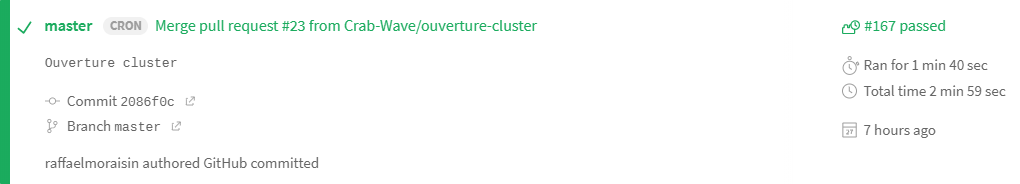
\includegraphics[width=17cm]{assets/presentation1/travis.png}
        \caption{Rapport des travaux de l'intégration continue sur le dernier changement}
      \end{figure}

    \clearpage
      
  \section{Méthodologies utilisées}

    \subsection{Avantages}
      Un des avantages de l'utilisation de l'intégration continue avec \textit{Travis CI} ainsi que l'utilisation des \textit{Pull Requests} et \textit{Issues} de \textit{GitHub} est que la branche principale du dépôt Git reste propre et fonctionnelle quoi qu'il arrive. Cela nous permet de toujours proposer un programme sans bugs majeurs (théoriquement).
      De plus, grâce à l'intégration continue et aux \textit{tests unitaires} produits avec le \textit{Test Driven Development}, nous pouvons développer les fonctionnalités d'ORA tout en évitant le fameux problème du "ça fonctionne sur mon PC", puisque des tests sont effectués à chaque nouveau commit sur différentes plateformes dans le \textit{Cloud}.

    \subsection{Inconvénients}
      Bien qu'en théorie les méthodes citées plus haut nous permettent d'être mieux organisé dans notre travail, en réalité c'est un peu plus complexe que cela. En effet, il faut être très rigoureux afin de suivre toutes les "consignes", ce qui peut être un peu compliqué par moment, surtout lorsque nous ne sommes pas à temps plein sur le projet. Par exemple nous n'avons pas réussi à suivre complètement les objectifs fixés lors des réunions pour les Sprints. Le Sprint 3 à ainsi été sauté à cause des périodes de partiels et nous nous sommes attribués des tâches à la volée, sans réelle organisation.
      Un autre défaut, cette fois-ci dû au fait de travailler grâce aux \textit{Issues} et \textit{Pull Requests} de \textit{Github}, est le fait que devoir faire réviser le code par une autre personne avant d'incorporer la fonctionnalité en question dans le projet peut parfois prendre du temps, ce qui peut ensuite mettre en retard toute une branche du projet. Aussi, le \textit{Test Driven Development} s'est avéré plus difficile à mettre en place que prévu. Étant donné que nous sommes habitués à écrire du code tout de suite, nous ne pensons pas forcément à écrire les tests en premier. De plus, en essayant d'écrire les tests en premier, il est difficile d'imaginer les tests que l'on pourrait faire étant donné que notre connaissance de l'environnement .NET est pour l'instant limitée.
    
  \clearpage
  \section{Prochaine Soutenance}
    \subsection{Tracker}
      Pour la prochaine soutenance, nous devons mettre en place le système d'authentification des Nodes comme mentionné précédemment. De plus, nous devons implémenter d'autres routes comme la route /nodes qui permettra de recevoir les informations d'un Node. Enfin, nous tenterons d'optimiser encore le Tracker en essayant par exemple différentes alternatives à la base de donnée LevelDB comme RocksDB ou HyperLevelDB, afin de déterminer laquelle elle est la plus performante, et si ce n'est pas LevelDB, afin d'améliorer la vitesse de réponse du Tracker.
    
    \subsection{Daemon}
      Pour la prochaine soutenance, le Daemon aura été complété à 50\%, c'est-à-dire qu'il pourra gérer une petite partie des fonctionnalités de ORA (comme créer un Cluster, etc\ldots) ainsi que synchroniser les données avec le Tracker de manière automatique. Pour cela nous utiliserons de l'IPC (Inter-process communication) avec le CLI, qui passera donc par le Daemon pour effectuer des actions. Nous utiliserons la librairie publique \surl{https://github.com/jacqueskang/IpcServiceFramework} pour celà, bien que ce soit sujet à changement.
    
    \subsection{API}
      D'ici la prochaine soutenance, l'API devra être complète à environ 80\%, ce qui signifie que la plupart des services et structures de données devront avoir été créées. Cela inclut donc tout ce qui est en rapport avec les Identités et les fichiers.
    
    \subsection{Core}
    
      \subsubsection{Data Management}
        Pour la prochaines soutenance, nous implémenterons l'Identity Management, le Node Management et le File Management.\newline Le premier permet de gérer l'organisation des utilisateurs pouvant avoir accès à un Cluster. En effet, chaque Cluster aura des administrateurs qui pourront enlever ou ajouter des Nodes de celui-ci et un propriétaire qui aura, en plus des droits d'administrateur, celui de pouvoir supprimer celui-ci.\newline
        Le second permet à l'utilisateur d'ajouter ou de supprimer une Node (machine de l'utilisateur). Elle permet aussi d'obtenir le nom de celle-ci.\newline
        Le dernier permet à l'utilisateur d'ajouter ou de supprimer un fichier ou un dossier sur un Cluster. Elle permet aussi d'obtenir le nom de celui-ci.
        
\clearpage

      \subsubsection{Compression}
        Pour la prochaine soutenance, nous implémenterons l'algorithme de compression Zstandard, établi par Facebook. Nous avions choisi cet algorithme car en plus d'être en licence libre, son ratio taux de compression/vitesse le situe parmi les algorithmes de compression les plus efficaces.
    
        \begin{figure}[H]
          \centering
             \scalebox{1.3}{\begin{tabular}{|l|l|l|l|}\hline
             \textbf{Compressor name} & \textbf{Ratio} &
             \textbf{Compression}     & \textbf{Decompress}                                           \\ \hline
              \textbf{zstd 1.3.4 -1}   & 2.877          & 470 MB/s             & 1380 MB/s            \\ \hline
                      zlib 1.2.11 -1   & 2.743          & 110 MB/s             & 400 MB/s             \\ \hline
                      brotli 1.0.2 -0  & 2.701          & 410 MB/s             & 430 MB/s             \\ \hline
                      quicklz 1.5.0 -1 & 2.238          & 550 MB/s             & 710 MB/s             \\ \hline
                      lzo1x 2.09 -1    & 2.108          & 650 MB/s             & 830 MB/s             \\ \hline
                      lz4 1.8.1        & 2.101          & 750 MB/s             & 3700 MB/s            \\ \hline
                      snappy 1.1.4     & 2.091          & 530 MB/s             & 1800 MB/s            \\ \hline
                      lzf 3.6 -1       & 2.077          & 400 MB/s             & 860 MB/s             \\ \hline
              \end{tabular}}
            \caption{Comparaison de plusieurs algorithmes de compression}
          \footnotesize{Source: \surl{https://facebook.github.io/zstd/}}
          \label{fig:zstd_comparison}
        \end{figure}
    
    \subsection{CLI}
      Pour la prochaine soutenance, comme inscrit dans le cahier des charges, nous prévoyons que 80\% du CLI soit développer. Cela implique que toutes les méthodes du Data Management créées entre la première et la deuxième soutenance seront implémentées dans celui-ci. Il permettra donc:
      \begin{itemize}
          \item de gérer les Clusters, que ce soit les fichiers qui lui sont attribués ou encore les Nodes qui les possèdent.
          \item de synchroniser les fichiers de tous les Clusters auxquels nous appartenons.
          \item et bien d'autre encore.
      \end{itemize}
    
    \subsection{GUI}
      Pour la prochaine soutenance 30\% du GUI doit être fait. Cela correspond à la création et la mise en place du projet et développement d'un début d'interface permettant de gérer les Clusters ainsi que les Nodes.
    
    \subsection{Site Web}
      Bien qu'une grande partie du site web aie été réalisée il manque actuellement du contenu. Il faudrait améliorer la partie présentation c'est-à-dire la reformuler et la développer, ainsi qu'écrire un script ou utiliser un outil qui va générer la page de documentation à partir des commentaires de documentations écrits dans notre code.
    
    \clearpage
    \section{Conclusion}
    Pour notre première soutenance, nous avons rempli tous les objectifs énoncés dans notre planning de réalisation. Cependant il faut noter que l'évaluation d'un pourcentage d'avancement n'est pas très facile et pas très objective. Il faut donc prendre ces pourcentages dans un intervalle de $\pm5\%$.\newline
    Ainsi nous avons estimer l'avancement des tâches suivantes:
    \begin{itemize}
      \item le Tracker est à 70\% opérationnel;
      \item le Core est réalisé à 45\%;
      \item l'API est liée au Core, mais certaines fonctionnalités de ce dernier ne sont pas nécessaires à être importés dans l'API comme le chiffrement ou la compression par exemple; De ce fait l'API est complétée à 50\%;
      \item le Daemon est créé et initialisé aux conformes de notre projet sans méthodes pour l'instant. On arrive donc à 10\%;
      \item pour le CLI, nous avons un début d'interface avec quelques méthodes utilisant toutes les méthodes du Core pouvant servir directement l'utilisateur, en plus du changement d'url. Nous arrivons donc à 20\%;
      \item le GUI n'a pas encore été commencé;
      \item le site web est opérationnel à 50\% : on peut voir une présentation du projet et de toute l'équipe mais aussi tous les liens utiles pour les développeurs ayant envie de reprendre une partie de notre code.
      \item pour ce qui est de \LaTeX, nous avons créé notre propre 
    \end{itemize}
    Nous travaillerons avec le même rythme et la même intensité en vue de la deuxième soutenance pour pouvoir remplir les objectifs mentionnés plus haut. 

    \begin{table}[H]
      \centering
      \scalebox{1.5}{\begin{tabular}{llll} \hline
        \multicolumn{1}{|l|}{Tâches}   & \multicolumn{1}{l|}{1}    & \multicolumn{1}{l|}{2}    & \multicolumn{1}{l|}{3}     \\ \hline
        \multicolumn{1}{|l|}{Tracker}  & \multicolumn{1}{l|}{70\%} & \multicolumn{1}{l|}{90\%} & \multicolumn{1}{l|}{100\%} \\ \hline
        \multicolumn{1}{|l|}{API}      & \multicolumn{1}{l|}{50\%} & \multicolumn{1}{l|}{80\%} & \multicolumn{1}{l|}{100\%} \\ \hline
        \multicolumn{1}{|l|}{Core}     & \multicolumn{1}{l|}{40\%} & \multicolumn{1}{l|}{70\%} & \multicolumn{1}{l|}{100\%} \\ \hline
        \multicolumn{1}{|l|}{Daemon}   & \multicolumn{1}{l|}{10\%} & \multicolumn{1}{l|}{50\%} & \multicolumn{1}{l|}{100\%} \\ \hline
        \multicolumn{1}{|l|}{CLI}      & \multicolumn{1}{l|}{20\%} & \multicolumn{1}{l|}{80\%} & \multicolumn{1}{l|}{100\%} \\ \hline
        \multicolumn{1}{|l|}{GUI}      & \multicolumn{1}{l|}{0\%}  & \multicolumn{1}{l|}{30\%} & \multicolumn{1}{l|}{100\%} \\ \hline
        \multicolumn{1}{|l|}{Site Web} & \multicolumn{1}{l|}{40\%} & \multicolumn{1}{l|}{70\%} & \multicolumn{1}{l|}{100\%} \\ \hline
        \multicolumn{1}{|l|}{\LaTeX}   & \multicolumn{1}{l|}{40\%} & \multicolumn{1}{l|}{70\%} & \multicolumn{1}{l|}{100\%} \\ \hline
      \end{tabular}}
    \end{table}
 
  \clearpage

  \section{Annexe}
    \subsection{Vocabulaire}
      \subsubsection{API RESTful}
        Une API compatible REST, ou « RESTful », est une interface de programmation d'application qui fait appel à des requêtes HTTP pour obtenir (GET), placer (PUT), publier (POST) et supprimer (DELETE) des données.
        
      \subsubsection{Endpoint}
        Un endpoint (littéralement point d'accès) est un point à partir duquel une API se connecte au logiciel.
        
      \subsubsection{Issues}
        Sur GitHub, les Issues permettent d'indiquer quelles sont les tâches à réaliser dans un projet, que ce soit des nouvelles fonctionnalités à implémenter ou bien des bogues à régler.
        
      \subsubsection{Pull Request}
        Une pull-request désigne tout simplement l'action qui consiste à demander au détenteur du dépôt original de prendre en compte les modifications que vous avez apportées sur votre fork et que vous souhaitez partager
        
      \subsubsection{TDD}
        Le Test-Driven Development (TDD), ou Développements Pilotés par les Tests en français, est une méthode de développement de logiciel qui consiste à écrire chaque test avant d'écrire le code source d'un logiciel, de façon itérative.
        
      \subsubsection{Travis CI}
        Travis CI est une plateforme d'intégration continue, elle nous permet de lancer automatiquement des travaux sur chaque \textit{commit}. On rappelle que nous avons réglé notre répertoire Git de sorte qu'il soit impossible de fusionner une branche avec la branche master si les travaux d'intégration continue ne passent pas sur cette branche.

\end{document}
